% =============================================
% Part 0.0 编辑个人信息
% =============================================

\newcommand{\department}{计算机科学与技术}		%在这里修改系别
\newcommand{\major}{计算机科学与技术}				%在这里修改专业
\newcommand{\class}{计类1707}					%在这里修改班级
\newcommand{\name}{	张谦益		}			%在这里修改姓名
\newcommand{\stuid}{ 			}				%在这里修改学号
\newcommand{\newdate}{			}				%在这里修改日期 yyyy-mm-dd
\newcommand{\loc}{			}					%在这里修改地点

% =============================================
% Part 0.1 编辑课程信息
% =============================================
\newcommand{\newcourse} {数据结构\LARGE{(C)}} %在这里修改成课程名称
\newcommand{\newtitle}{栈或队列的基本操作与应用} %在这里修改实验项目
\newcommand{\exptype}{计算机}

\newcommand{\grades}{}
\newcommand{\group}{无}

\newcommand{\tutor}{丁濛}
\newcommand{\onespace}{\hspace{1em} }
\begin{document}
\begin{titlepage}
	\centering
	\vspace*{1cm}
	{\fontsize{34pt}\baselineskip 实\onespace 验\onespace 报\onespace 告}\\
	\vspace{2cm}
	\fontsize{19pt}\baselineskip
	\makebox[30mm]{课程名称:}
	\underline{\makebox[75mm][c] {\newcourse} }
	\vskip 0.3cm
	\makebox[30mm]{实验项目:}
	\underline{\makebox[75mm][c] {\newtitle }}\\
	\vskip 0.3cm
	\makebox[30mm]{实验仪器:}
	\underline{\makebox[75mm][c]{ }}\\%在这里修改实验仪器
	\vskip 1cm

    \begin{table}[!htbp]
      \centering
      \sihao
      \begin{tabular}{| c | c | c | c | c | c |}
      	\hline
        项目 & 报告格式 & 写作质量 & 逻辑、注释质量、思想描述 & 复杂度分析 & 合计\\
        \hline
        
        百分比(\%) & 15 & 25 & 40 & 20  & 100 \\
        \hline
        得分	& {\gradeFormat } & {\gradeCode } & {\gradeComment}   & {\gradeComplex} & {\gradeTotal} \\
        \hline
      \end{tabular}
    \end{table}
     \Comments
    	
	\vskip 2cm

        \begin{table}[!tbhp]
            \centering
            \sanhao
            \begin{tabular}{ll}
                系\hspace{2em}别:	&	 \underline {\makebox[60mm][c]	{\department} 	} \\
                专\hspace{2em}业:	&	 \underline {\makebox[60mm][c] {\major}		} \\
                班级姓名:		&	\underline {\makebox[60mm][c] {\class\ \name\ }		} \\
                日\hspace{2em}期:	&	 \underline {\makebox[60mm][c]	{\newdate} 	} \\
                成\hspace{2em}绩:	&	 \underline {\makebox[60mm][c] {\grades}		} \\
                同组成员:		&	\underline {\makebox[60mm][c] {\group}		} \\
                指导教师:		&	\underline {\makebox[60mm][c] {\tutor}		} \\
            \end{tabular}
        \end{table}


%    
%    

\end{titlepage}

\newpage
% =============================================
% Part 2 Main document
% =============================================
\xiaosihao
\section{实验目的}
\begin{enumerate}
\item 熟练掌握栈和队列的基本操作原则;
\item 掌握栈和队列的顺序存储和链式存储实现方式;
\item 实现一个循环队列;(验证)
\item 会用栈解决实际问题。(设计、综合)
\end{enumerate}

\section{实验内容}
\subsection{项目一}
实现一个链式存储的栈结构并分析每个功能的复杂度,要求具有栈的基本功能。
\begin{enumerate}
\item 构造,析构;
\item Pop,Top,Push,size

\end{enumerate}

\subsection{项目二}
实现顺序存储的循环队列,并分析每个功能的复杂度,要求具有队列的基本功能。
\begin{enumerate}
\item 构造,析构;
\item EnQueue,DeQueue,Size
\end{enumerate}

\subsection{项目三}
利用栈,完成一个后缀四则表达式的计算,并返回结果。

\subsection{项目四}
完成上机平台上实验二的题目。

\section{实验过程}
\subsection{项目1}
大致思想 blablabla
\subsubsection{实验步骤}
\subsubsection{必要代码}
\lstinputlisting[language=C++]{code/main.cpp}
\subsubsection{实验结果}
	\begin{figure}[!bthp]
	\centering
        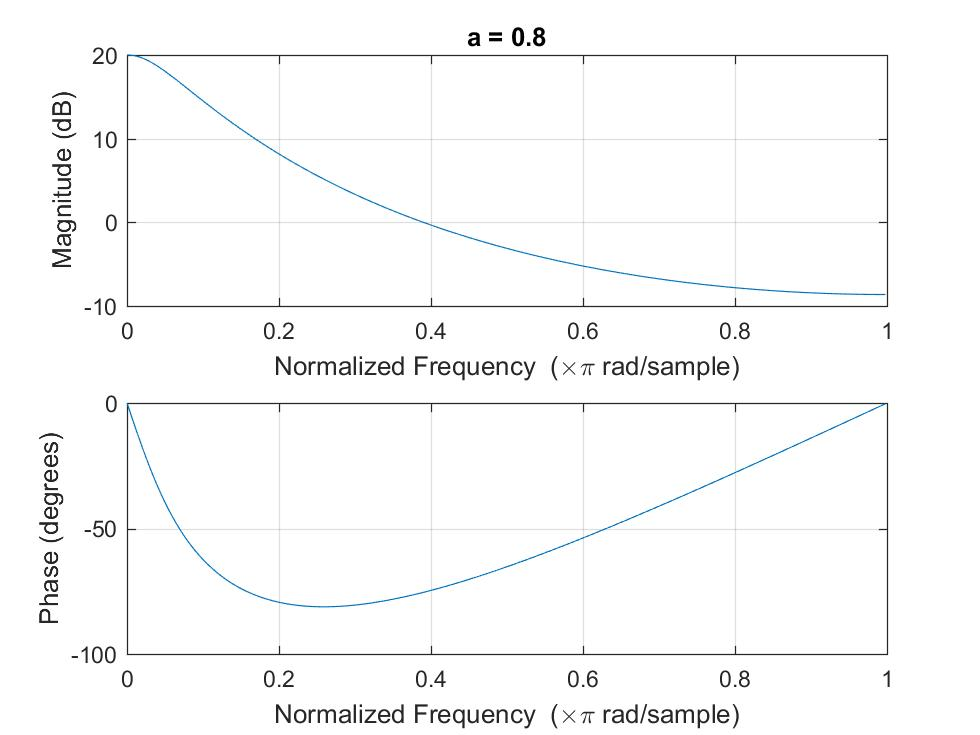
\includegraphics[width=0.6\linewidth]{02-1.jpg}
        \caption{D大调}
      \end{figure}

\subsection{项目2}
大致思想 blablabla sdfhasdfklj asd flas jkfjaksdf asd f
fasdf aksdjf klasj dfa
sdf
asdf

f
\subsubsection{实验步骤}
\subsubsection{必要代码}
\subsubsection{实验结果}

\subsection{项目3}
大致思想 blablabla
\subsubsection{实验步骤}
\subsubsection{必要代码}
\subsubsection{实验结果}

\subsection{项目4}

\section{实验总结}

\end{document}
